\documentclass[11pt]{article}

\usepackage{graphicx}
\usepackage[utf8]{inputenc}
\usepackage[margin=3.5cm]{geometry}
\usepackage{hyperref}
\usepackage{minted}
\graphicspath{{./images/}}

\title{
\includegraphics[scale=0.3]{logo.png} \\ \textbf{File Transfer Protocol}}
\author{Computer Networks\\ Bachelors in Informatics and Computing Engineering \\ \\ 3LEIC03\_G6 \\ \\ Tiago
Rodrigues up201907021@fe.up.pt \\ Mário Travassos up201905871@fe.up.pt  }
\date{\today}

\begin{document}

\maketitle

\newpage

\section*{Summary}

\paragraph{}This report will cover the second project proposed for the Computer Networks Curricular Unit, which had the objective of developing an application that would download files using the FTP (File Transfer Protocol) standard, along with setting up a network between the labs computers.

\paragraph{}The application supports both anonymous and authenticated downloads, and the arguments must be valid URL's, without the port.

\section*{Introduction}

\paragraph{}The second project had two main objectives: The development of the download application, and the configuration of the computer network. This report will examine both sections, detailing the architecture of the application and the setup used to launch the network. The application can be used to download files from any FTP server, since it adopts the standard URL syntax.

\paragraph{}The report is structured as follows: First, the application is described in detail, breaking down the architecture and the more relevant components. Then, a report of a successful download is made. After that, an analysis of the network will take place. Finally, a set of relevant attachments will be included.

\section*{Download Application}

\subsection*{Architecture}

\paragraph{}The application is simple by design. The way it operates internally resembles the way files were retrieved using the same protocol, in the first lab experiment that used \textbf{telnet}. It connects to the remote server using a socket, and after the connection is established, sends a set of FTP requests that will retrieve the desired file.

\subsubsection*{Program flow}

\paragraph{}The first two requests the program makes are authentication ones, which login the user. If the user does not specify a username and password in the URL, the default is ``anonymous'' and ``pass'', for the user and password respectively. If the login is successful, the program then requests the server to enter passive mode. The server's response to this command includes the IP address and the port for the file to be transferred from. The program determines this port, connects to it, and then asks the server to begin the transfer of the file specified in the URL. After the file is requested, the program reads the bytes from the socket, and writes them to the directory it was called from, with the same name as the transferred file. If at any point during execution an error occurs or the response from the server is not the expected one, the program terminates gracefully.

\subsubsection*{Main Modules}

\paragraph{}The program is logically divided in the following modules:

\begin{itemize}
    \item{parser: Responsible for decomposing the given URL and dividing it into the relevant tokens, saving them for later use.}
    \item{connection: Responsible for establishing a connection with the remote server.}
    \item{communication: Responsible for sending commands and reading responses, acting accordingly.}
    \item{file: Responsible for reading the incoming file and writing it onto the local machine.}
\end{itemize}

\paragraph{}There is also a shared file that includes common definitions like server response codes, and a main file that unites the modules described above.

\subsection*{Case study}

\paragraph{}The majority of the anonymous download tests were done by downloading from the server at \textbf{ftp.up.pt}, but since it only supports anonymous login, the authenticated tests were done using the server at \textbf{netlab1.fe.up.pt}, using the username \textbf{rcom} and password \textbf{rcom}. All of them were successful.

\paragraph{}The application allows the user to see the information he gave in the URL separated into the components, to check if it is correctly formatted. Also, in the event of a failure, the application shows the bad response code and message that led to the termination.

\section*{Network Configuration and Analysis}
\paragraph{}Part two of our assignment consisted in configuring a small local network as demonstrated in the picture below:

\begin{figure}[h]
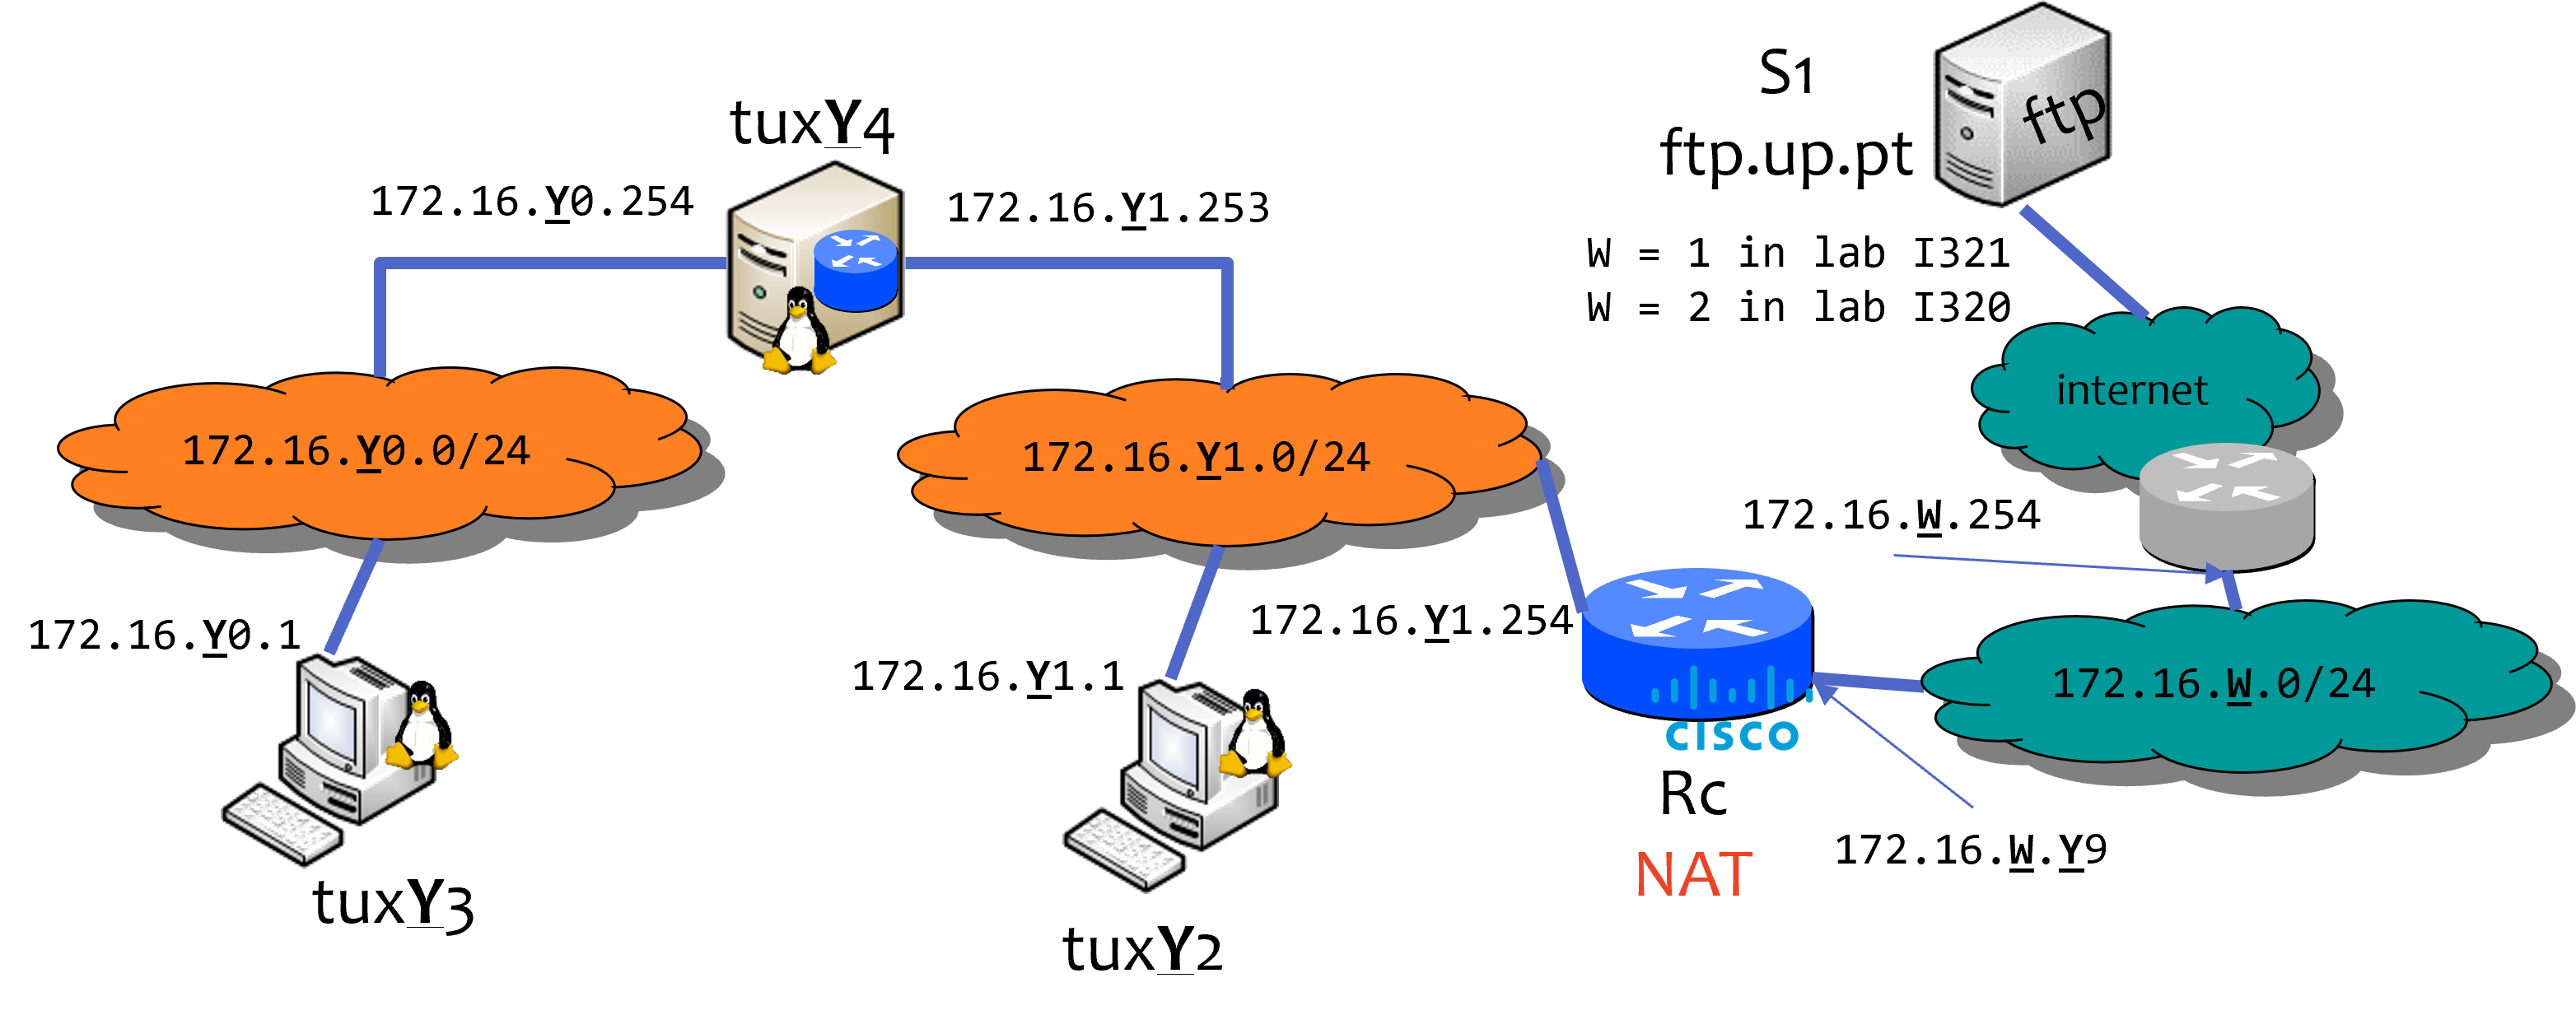
\includegraphics[scale=0.6]{images/net-complete.png}
\centering
\end{figure}

\paragraph{}In this image, \textbf{Y} is the lab bench number, (which in our case was 4), and \textbf{W} has a value depending on the lab we were working in. In our case, since we were working in lab I320, said value was 2.

\paragraph{}In order to correctly configure this network, we followed 4 experiment guides. Our experience will be described below.

\subsection*{Experiment 1:}

\paragraph{}Our goal in this experiment was to configure the ip address of tux43 and tux44, and connect those to a switch, which resulted in the following configuration:

\begin{figure}[h]
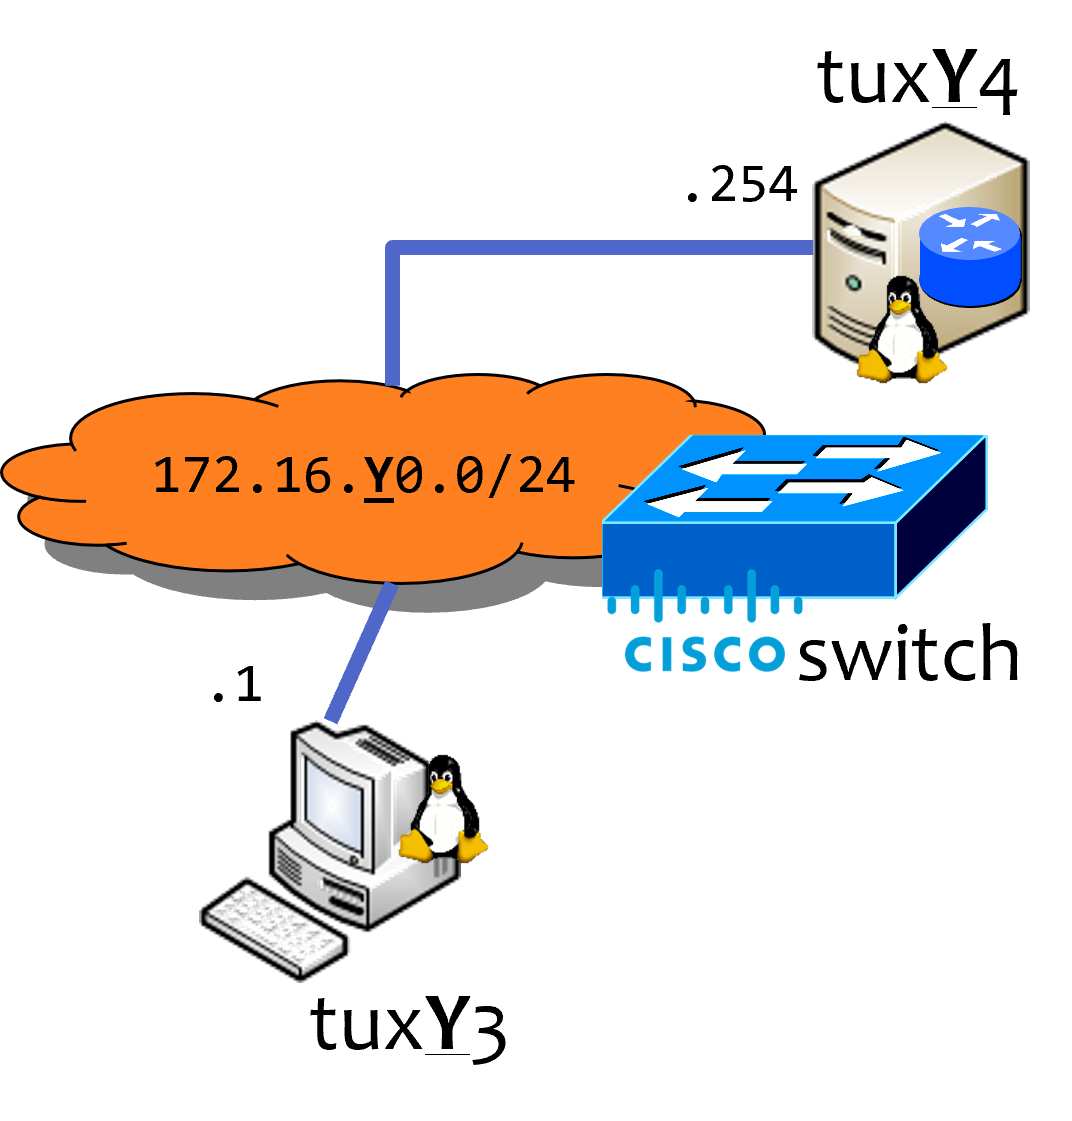
\includegraphics[scale=1]{images/net-exp1.png}
\centering
\end{figure}

\paragraph{}The steps we followed were as follows:

\begin{itemize}
    \item We disconnected the switch from netlab, cleaned the router and switch configurations, restarted the computers and connected the eth0 interfaces of tux43 and tux44 to it:
    \begin{itemize}
        \item port 1 - tux43;
        \item port 2 - tux44.
    \end{itemize}
    \item We configured tux43 and tux44 to have the IP addresses shown in the image above (replacing Y with 4), and defined the network 172.16.40.0/24, using ifconfig and the route commands;
    \item We noted down the IP and MAC addresses of the network interfaces on both tuxes, for later analysis;
    \item We pinged the computers from one another to verify the connectivity between them.;
    \item We inspected the forwarding table and the ARP table;
    \item We deleted the ARP table entries in tux43;
    \item After starting Wireshark in eth0 of tux43 and starting the packet capturing process, we pinged tux44 from tux43 for a few seconds;
    \item After saving the wireshark log, we analized it, in order to gain some insight into the inner workings of the network we just set up.
\end{itemize}

\subsection*{Experiment 2:}

\paragraph{}Our goal in this experiment was to configure the two virtual lands in our bench's switch, as demonstrated by the following diagram:

\begin{figure}[h]
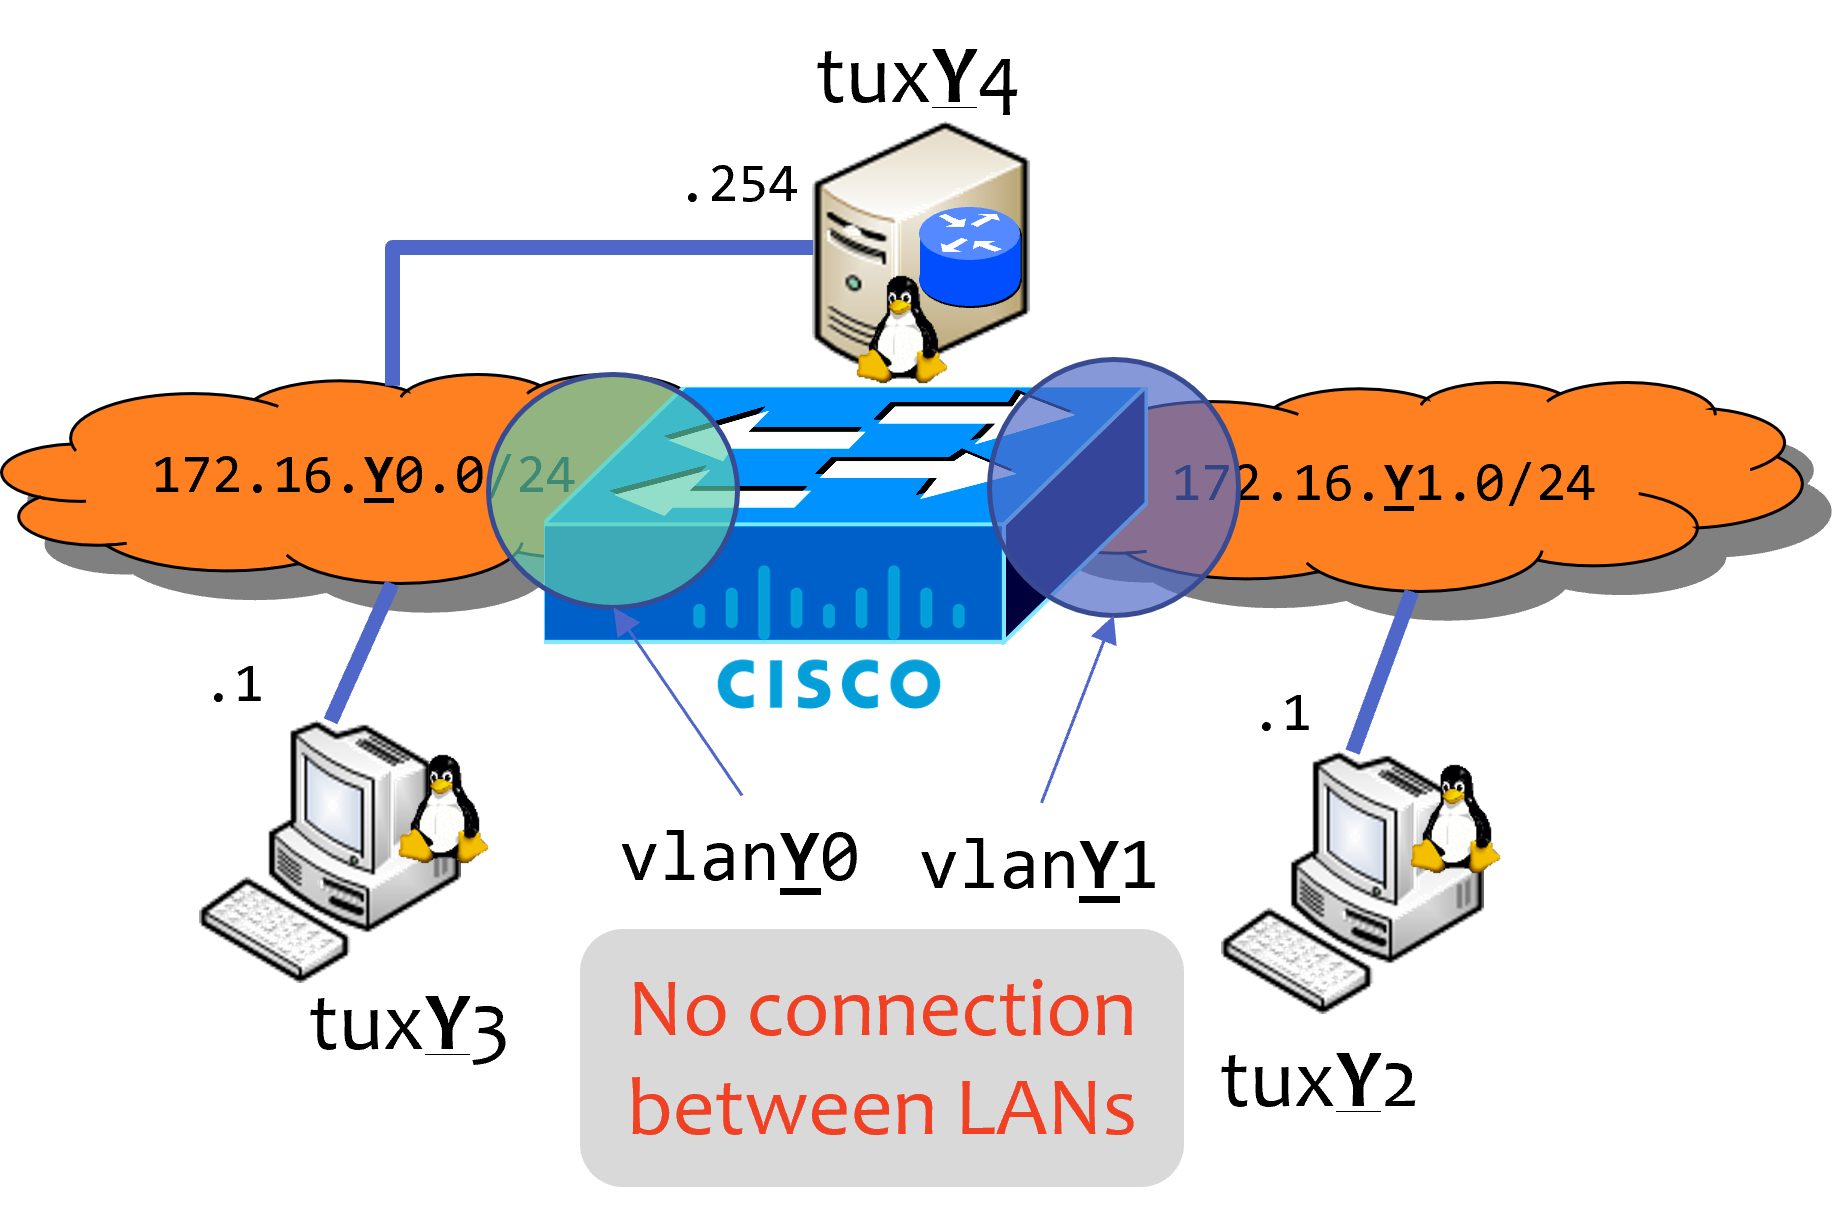
\includegraphics[scale=1]{images/net-exp2.png}
\centering
\end{figure}

\paragraph{}The steps we followed were as follows:

\begin{itemize}
    \item Connected eth0 of tux42 to port 13 of the router and configured its network (taking note of its IP and MAC addresses, just as before);
    \item Created the vlans 40 and 41 in the switch and added their corresponding ports (1 and 2 to vlan40; 13 to vlan41);
    \item Started a Wireshark capture at eth0 of tux43, from where we pinged tux44 and tux42, saving the log after pinging;
    \item Started Wireshark captures in eth0 of tux43, eth0 of tux44 and eth0 of tux42;
    \item We made a ping with the broadcast flag to 172.16.40.255 and saved the resulting logs;
    \item We repeated the previous two steps, but this time, pinging 172.16.41.255.
\end{itemize}

\subsection*{Experiment 3:}

\paragraph{}During experience 3, we focused on analyzing and setting up a configuration file for a Cisco Router. Our goal was to better understand and to prepare to implement the following network diagram:

\begin{figure}[h]
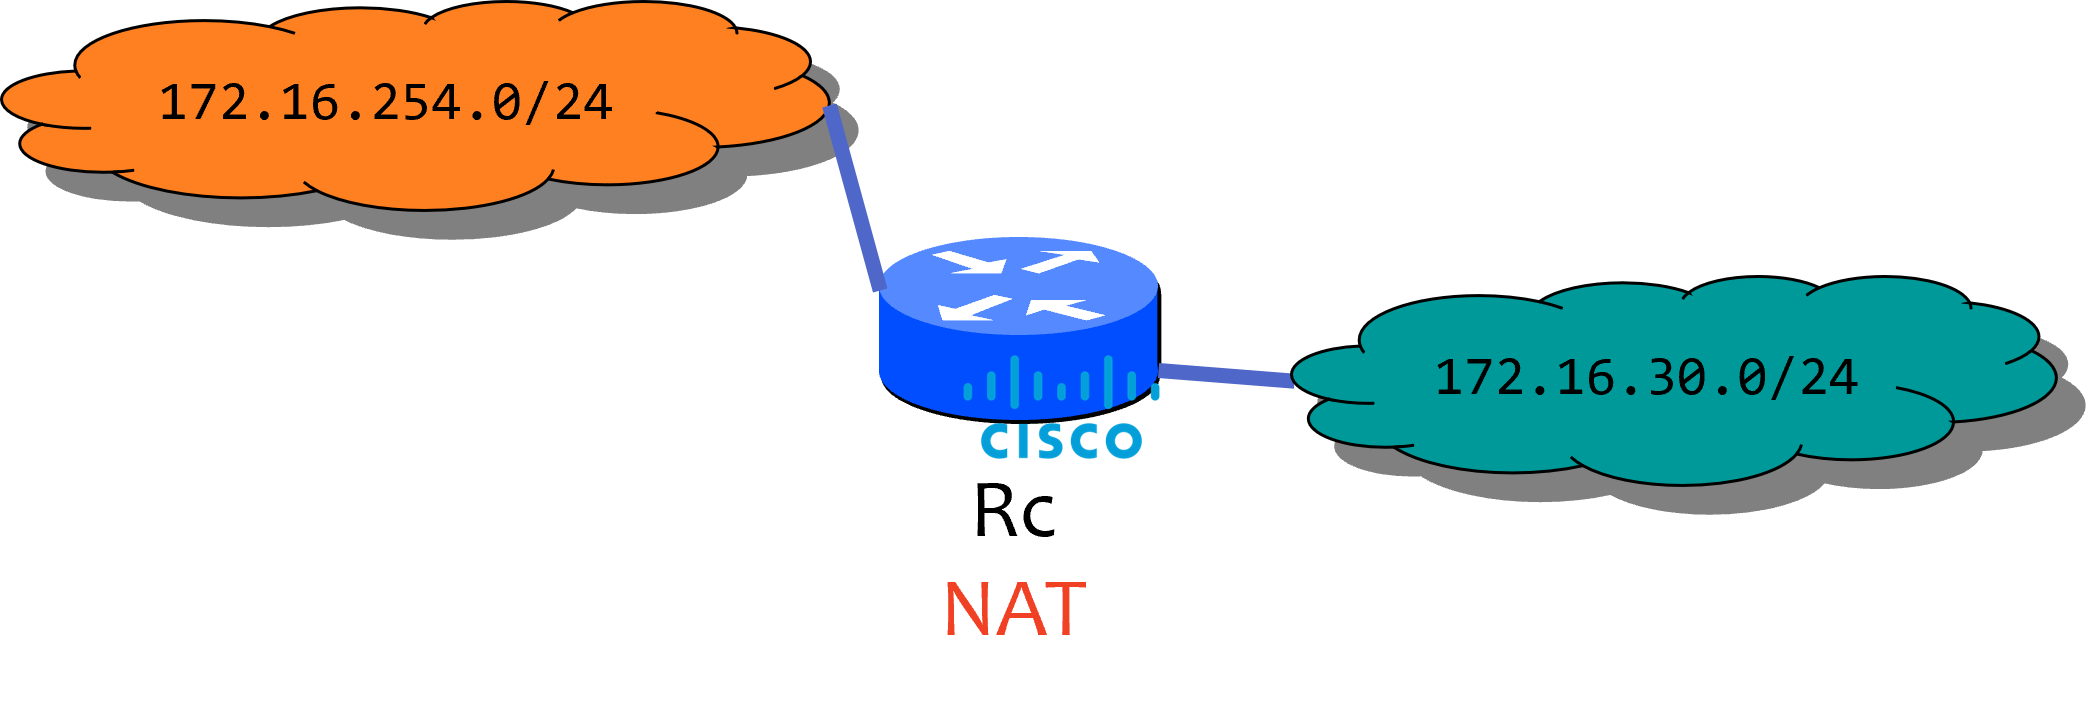
\includegraphics[scale=1]{images/net-exp3.png}
\centering
\end{figure}

\paragraph{}The steps we followed were as follows:

\begin{itemize}
    \item Having been provided a configuration file for a Cisco router that is doing NAT and routing on its interfaces (as represented in the above figure), we analyzed its configuration file;
    \item With the help of the Cisco IOS documentation for the Basic Router Configuration, we checked, changing values where necessary, the following configurations:
        \begin{itemize}
            \item Router name;
            \item Ethernet Ports available and of what type (in our case, only fast-ethernet);
            \item Configured IP addresses and netmask of ports;
            \item Configured routes.
        \end{itemize}
    \item We took a closer look into the router's NAT configuration, namely the fields related to the interfaces which are connected to the internet, the number of IP addresses available for NATing and router overloading.
\end{itemize}

\paragraph{}After the previous steps, we ended up with the configuration file which we appended to this report in the Annexes section.

\subsection*{Experiment 4:}

\paragraph{}Experience 4 consisted of applying the configuration created during experience 3, on top of the work developed in labs 1 and 2.

\paragraph{}This experience was devided into two smaller goals: \textbf{Configuring the Linux Router} and \textbf{Configuring the Cisco Router}.

\subsubsection*{Configuring the Linux Router}

\paragraph{}This procedure is geared towards correctly configuring the following network:

\begin{figure}[h]
    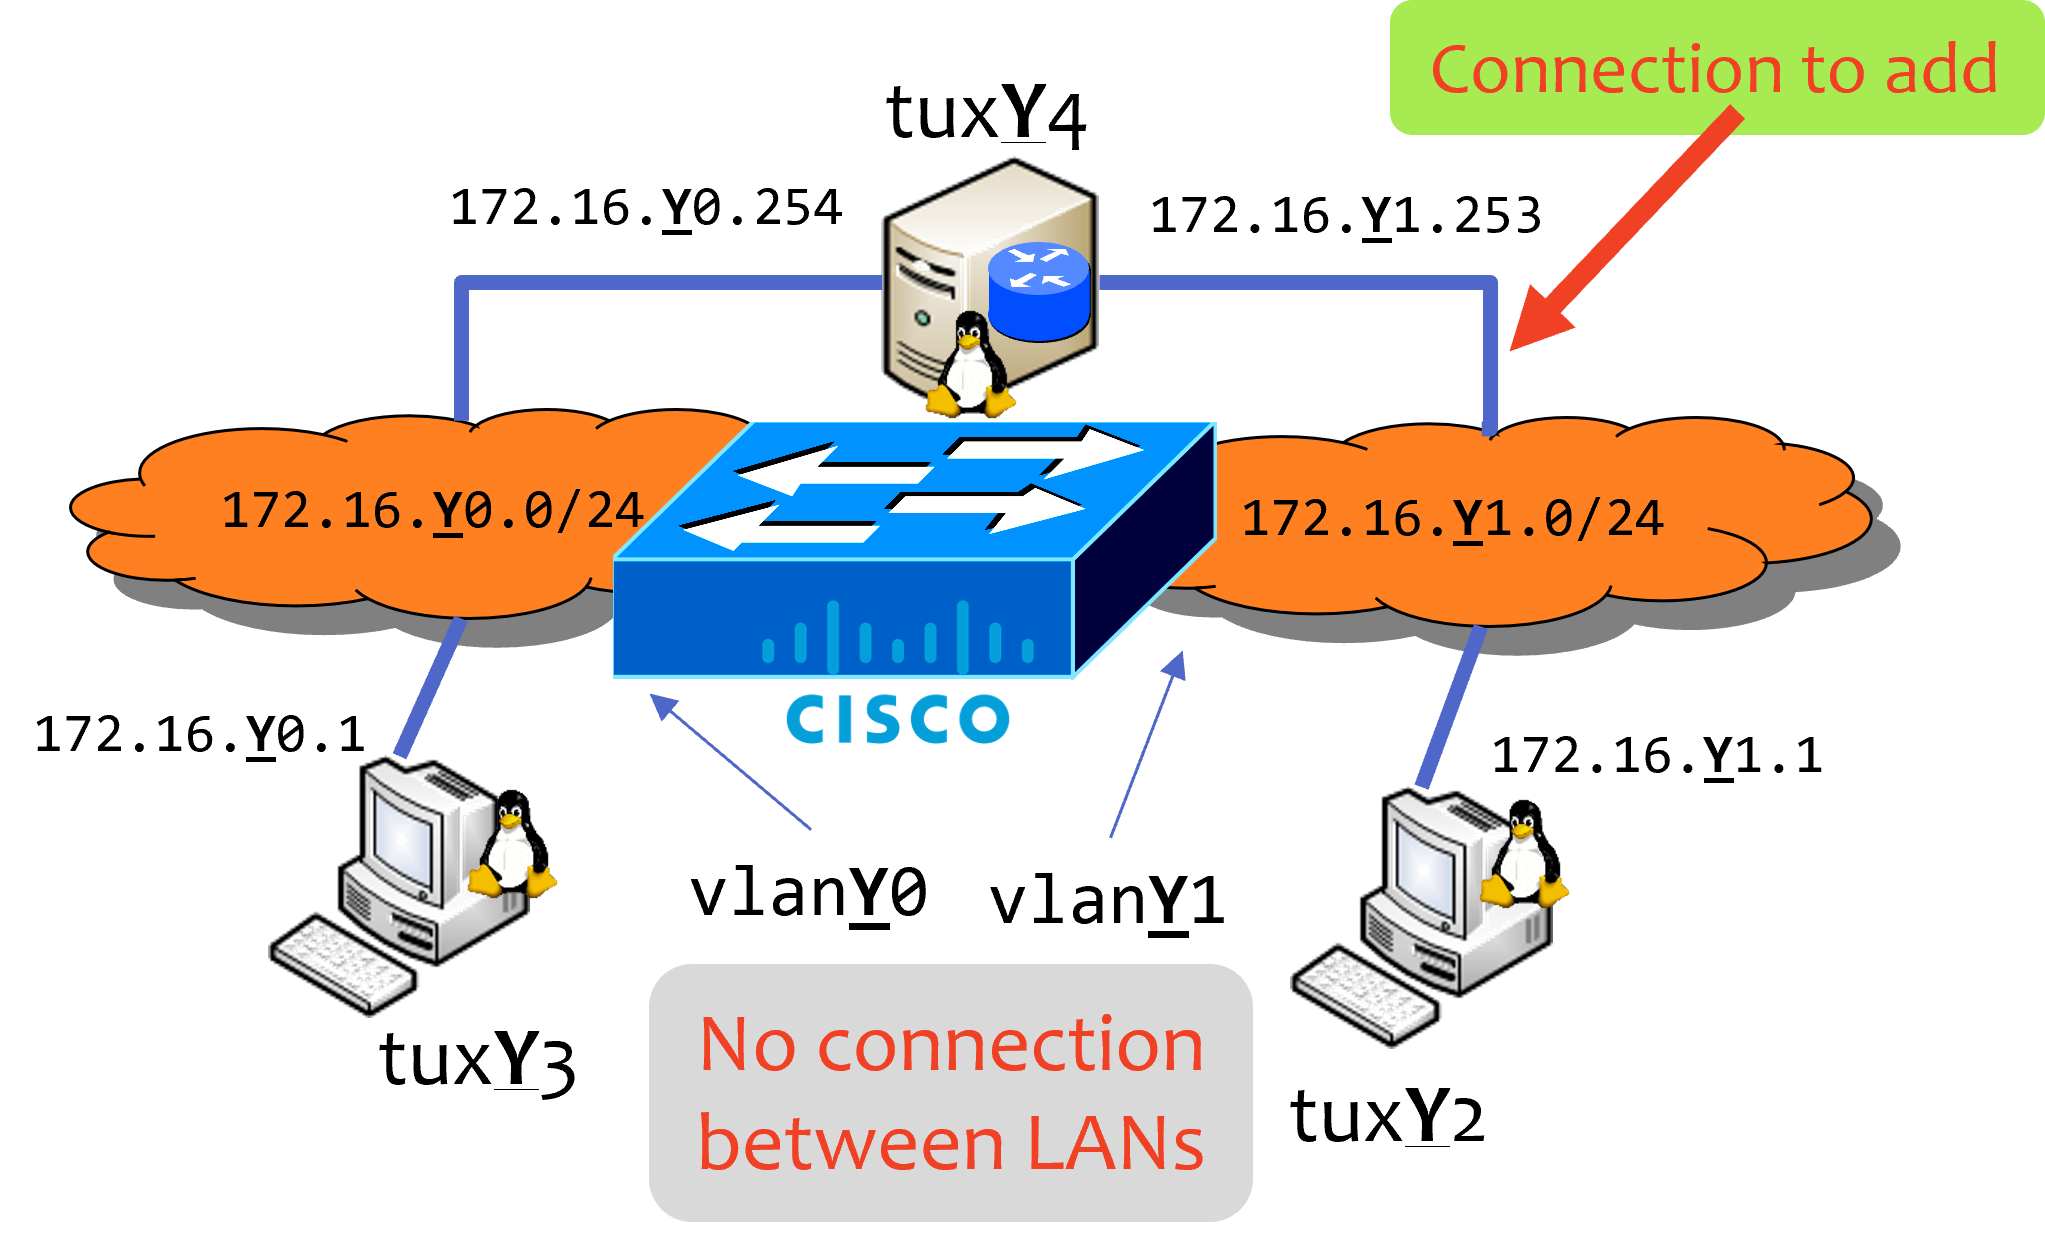
\includegraphics[scale=1]{images/net-exp4-1.png}
    \centering
\end{figure}

\paragraph{}The steps we followed for this first procedure were as follows:

\begin{itemize}
    \item We connected a cable from tux44's eth1 interface to port 14 of the switch, and added that port to vlan41, following the same procedure used in experiment 2;
    \item Configured tux44's eth1 interface's IP address to be the same as represented in the image above (172.16.41.253/24);
    \item Enabled IP forwarding and disabled ICMP echo ignore broadcast, on tux 44;
    \item Took note of the IP and MAC addresses in tux44, for both of its interface, for further study;
    \item Configured the routes in tux43 and tux42, in order for them to reach one another;
    \item Started a wireshark capture at tux43, from where we pinged the other network interfaces, 172.16.40.254, 172.16.41.253, 172.16.41.1. We saved the log for later reference;
    \item Started a capture in tux44, on both of its interfaces, eth0 and eth1;
    \item We cleared the ARP tables of all 3 tuxes;
    \item From tux43 we pinged tux42 for a few seconds, and stopped the capture in tux44, saving the logs.
    \item Inside Wireshark, we opened the last capture last capture log and viewed the packets from each interface using, in the display filter, the "test frame.interface\_id == X" filter, where X is the number of the interface we want to study.
\end{itemize}

\subsubsection*{Configuring the Cisco Router}

\paragraph{}In this step of the experiment, we seek to connect our setup to the world wide internet, as illustrated by the image below:

\begin{figure}[h]
    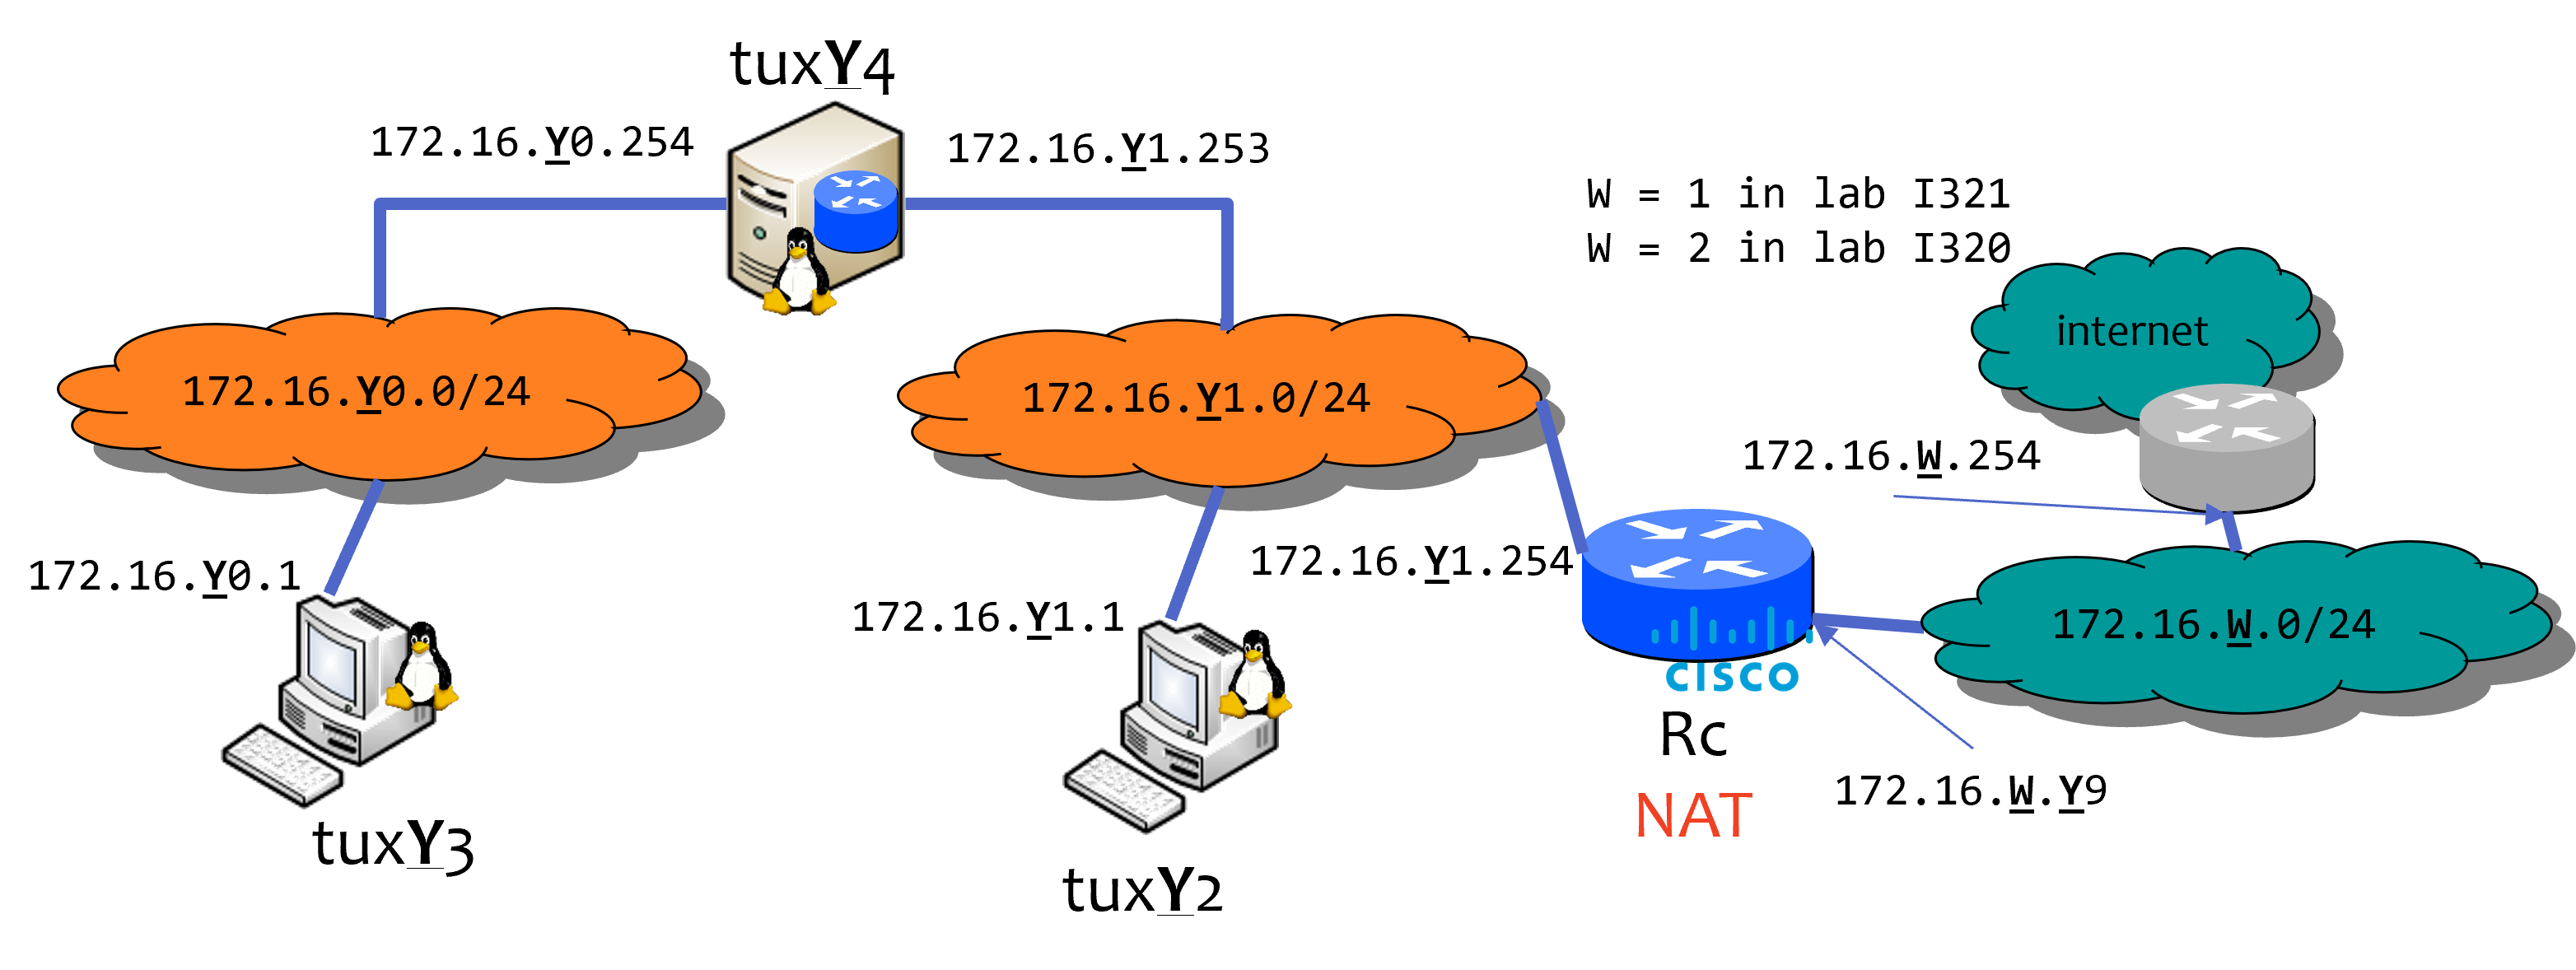
\includegraphics[scale=1]{images/net-exp4-2.png}
    \centering
\end{figure}

\paragraph{}The steps we followed for the second procedure were as follows:

\begin{itemize}
    \item Connect the FE0 interface of the Cisco Router to the Lab Router, and the FE1 interface to the Switch;
    \item Configured the switch's port to be on the correct vlan;
    \item We connected to the router via serial port, and applied our configuration file on the router, thereby configuring it;
    \item To verify the connectivity, we did a ping from the Cisco Router to all the tuxes, to 172.16.2.254 and to 104.17.113.188 (on the internet);
    \item We set tux42 and tux44's default gateways to the Cisco Router (172.16.41.254);
    \item Pinged 172.16.2.254 from tux43;
    \item Pinged 104.17.113.188 (the internet) from tux43.
\end{itemize}

\subsubsection*{Testing our network}

\paragraph{}This marks the end of our experiments, thereby allowing us to successfully run our download application, in order to retrieve content from an FTP server on the internet, namely FEUP's FTP server.

\paragraph{}In preparation for our final demonstration, we prepared a few bash scripts, and some configuration files which when executed would run crucial commands to set up the network just as it was set up after this configuration, which will be appended in the Annexes section of this document. These files are the following:

\begin{itemize}
    \item tux42\_conf.sh - to be run inside tux42;
    \item tux43\_conf.sh - to be run inside tux43;
    \item tux44\_conf.sh - to be run inside tux44;
    \item vlan.conf - vlan configuration commands to be run inside the switch console, accessible via serial port;
    \item router.conf - router configuration commands to be run inside the cisco router console, accessible via serial port.
\end{itemize}

\section*{Conclusions}

\paragraph{}The implemented download application achieved the proposed results, being able to download files from any FTP server using the FTP standard. More importantly, the standard was very well understood.

\paragraph{}The 2nd part of the project allowed us to get some hands-on experience, giving us the chance to apply the theoretical knowledge we have acquired during our classes to a real-life example, albeit a simplified, albeit to some extent convoluted. This also allowed us to gain a better understanding of how networks operate, and some insight into how this process may be automated in order to provide the end user with a more streamlined experience, giving us a small taste of how the inner workings of technologies which abstract and automate some of this configuration steps, such as DHCP, might look like.

\paragraph{}Furthermore, in order to simplify our reconfiguration process, we found ourselves dusting off some very rudimentary knowledge of bash scripting we had laying around. This was but a byproduct of the way in which the assignment was structured, but a well welcomed one. After getting the network up an running, we were able to run our download application from part 1, in order to download files from the faculty's ftp server, seeing the fruits of our hard labour.

\section*{References}

\begin{itemize}
    \item{RFC959 - File Transfer Protocol: \url{https://www.rfc-editor.org/info/rfc959}}
    \item{RFC1738 - Uniform Resource Locator (URL): \url{https://www.rfc-editor.org/info/rfc1738}}
\end{itemize}

\newpage

\section*{Annexes}

\subsection*{Annex I - Application Source Code}

\subsubsection*{communication.c}

\inputminted{c}{communication.c}

\newpage

\subsubsection*{communication.h}

\inputminted{c}{communication.h}

\newpage

\subsubsection*{connection.c}

\inputminted{c}{connection.c}

\newpage

\subsubsection*{connection.h}

\inputminted{c}{connection.h}

\newpage

\subsubsection*{defines.h}

\inputminted{c}{defines.h}

\newpage

\subsubsection*{download.c}

\inputminted{c}{download.c}

\newpage

\subsubsection*{file.c}

\inputminted{c}{file.c}

\newpage

\subsubsection*{file.h}

\inputminted{c}{file.h}

\newpage

\subsubsection*{parser.c}

\inputminted{c}{parser.c}

\newpage

\subsubsection*{parser.h}

\inputminted{c}{parser.h}

\newpage


\subsection*{Annex II - Configuration Commands}


\subsection*{tux42conf.sh}

\inputminted{bash}{tux42conf.sh}

\newpage

\subsection*{tux43conf.sh}

\inputminted{bash}{tux43conf.sh}

\newpage

\subsection*{tux44conf.sh}

\inputminted{bash}{tux44conf.sh}

\newpage

\subsection*{vlan.conf}

\inputminted{text}{vlan.conf}

\newpage

\subsection*{router.conf}

\inputminted{text}{router.conf}

\newpage


\end{document}
